

\begin{wrapfigure}[0]{r}[-5cm]{0.5cm}
 \vspace{-6cm}
  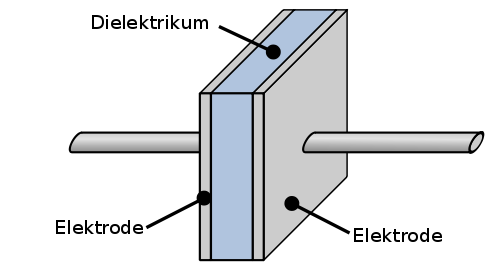
\includegraphics[scale=0.45]{Kondensator/Bilder/Kondensator.png}
 \vspace{-6cm}
\end{wrapfigure}

\section*{Theorie- und Prüfungsfragen}



%\loesung{
%\begin{figure}[H]
%\centering
%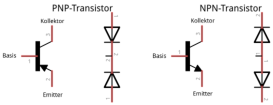
\includegraphics[scale=3]{Transistor/Bilder/PNP_NPN.pdf}
%\caption{1 und 2 - NPN- und PNP-Transistor}
%\end{figure}
%}


\mucho{1}{TC206}
{
Drei Kondensatoren mit den Kapazitäten $C_1 = 0,1\mu F$, $C_2 = 150nF$ und $C_3 = 50000pF$ werden parallel geschaltet. Wie groß ist die Gesamtkapazität?
}%Frage
{$0,027\mu F$}%A
{$0,255\mu F$}%B
{$0,3\mu F$}%C
{$2,73nF$}%D
{C; $C_g = 100nF + 150nF + 50nF = 300nF = 0,3\mu F$}%Lösung


\mucho{2}{TD105}
{
Berechnen Sie die Gesamtkapazität der gemischten Schaltung.\\
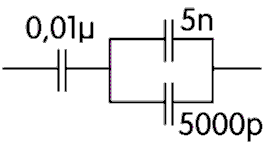
\includegraphics[scale=0.35]{Kondensator/Bilder/TD105.png}
}%Frage
{$0,015nF$}%A
{$5nF$}%B
{$7,5nF$}%C
{$10nF$}%D
{B; $C_g = \dfrac{C_1 \cdot C_{2+3}}{C_1 + C_{2+3}} = \dfrac{10nF \cdot (5nF + 5nF)}{10nF + (5nF + 5nF)} = 5$}%Lösung

\mucho{3}{TD106}
{
Berechnen Sie die Gesamtkapazität der gemischten Schaltung. Gegeben: $C1 = 0,02\mu F$; $C2 = 10nF$; $C3 = 10000pF $ \\
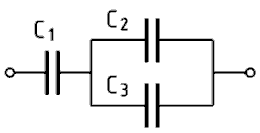
\includegraphics[scale=0.35]{Kondensator/Bilder/TD106.png}
}%Frage
{$2,5nF$}%A
{$5nF$}%B
{$10nF$}%C
{$40nF$}%D
{C; $C_g = \dfrac{C_1 \cdot C_{2+3}}{C_1 + C_{2+3}} = \dfrac{20nF \cdot (10nF + 10nF)}{20nF + (10nF + 10nF)} = 10nF$}%Lösung

\mucho{4}{TD107}
{
Berechnen Sie die Gesamtkapazität der gemischten Schaltung. Gegeben: $C1 = 0,01 \mu F$; $C2 = 10 nF$; $C3 = 5000 pF$\\
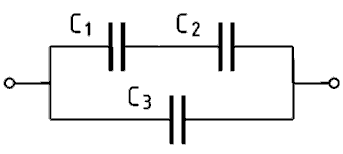
\includegraphics[scale=0.3]{Kondensator/Bilder/TD107.png}
}%Frage
{$2,5 nF$}%A
{$5 nF$}%B
{$10 nF$}%C
{$0,015 nF$}%D
{C; $C_g = \dfrac{C_1 \cdot C_2}{C_1 + C_2} + C_3 = \dfrac{10nF \cdot 10nF}{10nF + 10nF} + 5nF = 10nF$}%Lösung

\mucho{5}{TC208}
{Mit zunehmender Frequenz}%Frage
{steigt der Wechselstromwiderstand des Kondensators.}%A
{sinkt der Wechselstromwiderstand des Kondensators.}%B
{steigt der Wechselstromwiderstand des Kondensators bis zu einem Maximum und sinkt dann wieder.}%C
{sinkt der Wechselstromwiderstand des Kondensators bis zu einem Minimum und steigt dann wieder.}%D
{B; $X_C = \dfrac{1}{2\pi \cdot f \cdot C}$}%Lösung


\mucho{6}{TC201}
{Welche Aussage zur Kapazität eines Plattenkondensators ist richtig?}%Frage
{Je größer die angelegte Spannung ist, desto kleiner ist die Kapazität.}%A
{Je größer die Dielektrizitätszahl ist, desto kleiner ist die Kapazität.}%B
{Je größer die Plattenoberfläche ist, desto kleiner ist die Kapazität.}%C
{Je größer der Plattenabstand ist, desto kleiner ist die Kapazität.}%D
{D}%Lösung

\mucho{7}{TC202}
{Ein Bauelement, bei dem sich Platten auf einer isolierten Achse befinden, die zwischen fest stehende Platten hineingedreht werden können, nennt man}%Frage
{Drehkondensator.}%A
{Tauchkondensator.}%B
{Keramischer Kondensator.}%C
{Rotorkondensator.}%D
{A}%Lösung

\mucho{8}{TC207}
{Bei welchem der folgenden Bauformen von
Kondensatoren muss beim Einbau auf die
Polarität geachtet werden?}%Frage
{Elektrolytkondensator}%A
{Keramischer Kondensator}%B
{Styroflexkondensator}%C
{Plattenkondensator}%D
{A}%Lösung

\mucho{9}{TC203}
{Welche Kapazität hat der abgebildete Kondensator?\\
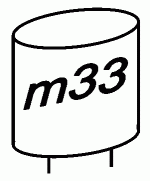
\includegraphics[scale=0.3]{Kondensator/Bilder/TC203.png}
}%Frage
{$3,3\mu F$}%A
{$33\mu F$}%B
{$33000\mu F$}%C
{$330\mu F$}%D
{D}%Lösung

\mucho{10}{TC205}
{Welche Kapazität hat der abgebildete Kondensator?\\
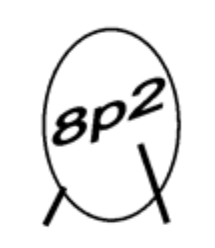
\includegraphics[scale=0.9]{Kondensator/Bilder/TC205.png}
}%Frage
{$820pF$}%A
{$8,2pF$}%B
{$82pF$}%C
{$0,82pF$}%D
{B}%Lösung